 \chapter[RICH]{RICH
\footnote{
  $CVS~revision~ $Id: rich.tex,v 1.1 2004/03/19 15:58:17 reitz Exp $ $
}
\footnote{Authors: B.Reitz \email{reitz@jlab.org}}
}
\label{sec:rich}

\section{Purpose and Layout} 

The Hall A RICH detector is designed to be used for particle identification purposes, mainly 
to identify kaons in a large background of pions and protons. The detector can be mounted in
the detector stack of the left HRS, between the trigger scintillator planes S1 and S2 (S2m),
together with the two Aerogel Cherenkov detectors.

Its design is conceptional identical 
to the CERN Alice HMPID detector \cite{Beole:1998yq}, but adapted to the special needs
of the Hall A environment.
A detailed description of the Hall A RICH detector can be found in \cite{hallarep02}.
The RICH has a proximity focusing geometry (no mirrors involved) which makes the 
detector compact (total thickness less than 50 cm) and relatively thin (18\% $X_0$).
Figure \ref{fcsirich.fig} shows the working principle of the adopted solution.
The Cherenkov effect takes place in the liquid freon 
when a charged particle 
crosses it.
The liquid radiator, 1.5 cm thick, 
is housed in a vessel made of NEOCERAM\footnote{NEOCERAM is
a glass-ceramic material with mechanical and thermal properties
almost identical to quartz.}    
on all sides but
the exit window which is made of pure quartz, 
0.5 cm thick. 
The use of a liquid radiator has been imposed by the momentum range (around
 2 GeV/c) of the particles to be identified.
The Cherenkov photons, emitted along a conical surface,
are refracted by the 
freon-quartz-methane interfaces and strike 
a pad plane after traveling a proximity gap 
of 10 cm filled with methane.

\infolevfour{
\begin{figure}[htb]
\begin{center}
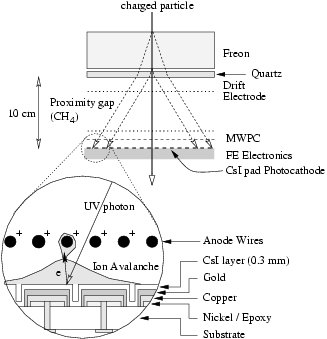
\includegraphics[angle=0, totalheight=9.cm]{freon-csi-rich} 
  \caption{\it Working principle of the freon CsI proximity focusing RICH.}
  \label{fcsirich.fig}
\end{center}
\end{figure}
}

The pad plane
 is covered by a thin substrate of CsI which
acts as photon converter. The emitted photo-electron is
accelerated by an electrostatic field (2100~V$/2$~mm) 
between the pad plane and
an anode wire plane in front of the pads,
 forming a MWPC (Multi Wire Proportional Chamber). 
While the anode wires collect the electron avalanche, the counterpart 
ions are collected by clusters of pads, each of which is connected to the
input channel of a multiplexed sample-and-hold electronics, housed on the
back of the pad plane.
At the end of this process, the
clusters of pads hit by the photons should be
scattered around a ring (ellipse) while 
one cluster coming from the charged particle track
should be located in the central region of the ring.
A drift electrode operated at 250~V and located close to the quartz window,
prevents electrons produced by ionization of the counting gas by charged 
particles in the proximity gap from reaching the MWPC. The MWPC of the RICH detector 
has to be operated with pure methane to achieve the 
designed performances. The first stage of front-end electronics is mounted on the 
backside of the detector. \infolevone{
Table \ref{rich_list.tab} presents a detailed list of the RICH components.  

\begin{table}
{\small
  \begin{center}
  \caption{Detailed list of the RICH components.}
  \label{rich_list.tab}
  \begin{tabular}{ll} 
    \\
    \hline 
    RICH size        & $50\times 210 \times 50$~cm$^3$ \\
    Optics           & proximity focusing \\
    Radiator         & 15 mm of liquid freon (C$_6$F$_{14}$) $n=1.28$\\
    Quartz window    & 5 mm, $n=1.56$ \\
    Position detector& MWPC, with one cathode of pads,
                       size: $1920\times403$~mm$^2$,
                       anode\\ 
                     &  wire pitch: 4.2 mm, anode-cathode gap: 2 mm,
                       amplification gas:\\ 
                     & CH$_4$ at STP, operating voltage: 2 kV \\
    Pad surface      & 3 pad planes, 
                       $630\times400$~mm$^2$ each;
                       11520 pads, $8\times8.4$~mm each\\
    Photon converter & 300~nm of CsI coating the pad surface \\
    Electronics      & analog, charge sensitive sample
                       and hold, 11520 channels\\
                     &  multiplexed in 48 ADCs \\
    \hline
  \end{tabular}
  \end{center}
}
\end{table}
}

The RICH detector is mounted together with the standard HRS detector package 
in the shield hut of the left HRS in Hall A. For the operation of the RICH
detector the following systems need to be installed in Hall A.

\infolevone{
\section{Description of Components}

\subsection{Gas System} 

\begin{safetyen}{10}{5}The MWPC needs to be flushed with ultra high purity
methane, when the detector is operated or in stand-by, or with 
an ultra high purity inert gas (argon) when the RICH is not used.\end{safetyen}
If the detector is not flushed with clean gas for extended periods,
there is a risk of damage or degradation of the CsI photo-cathode.
The choice of using methane as counting gas is based on experience with 
comparable detectors at CERN and STAR, it is the optimal choice concerning 
detector efficiency. \begin{safetyen}{10}{5} However, methane like other hydrocarbons, is flammable,
so care must be taken to mitigate the hazards involved with its use.\end{safetyen}
The methane supply is an addition to 
the Hall A Wire Chamber Gas System HAWGS\cite{Hawgswww}. The complete gas system is 
described elsewhere in this document.
Devices to monitor water and oxygen contaminations 
and filters to clean out oxygen contaminations are installed in the lines close to the 
detector itself. 
The flow is restricted by \begin{itemize}
\item an Excess-Flow valve (maximum flow 4~l/min, standard flow is 1~l/min)
located in each gas supply line just prior to the entry to the gas shed;
\item by the mass-flow control system which meters the gas delivered out of the 
gas shed to the two shield houses. 
\end{itemize}
Metal tubing is used throughout the whole gas system, besides 10~m of 
nylon tubing around the pivot and in the flexible cable tray. 
The remote controls for the 
RICH gas system is integrated into the standard Hall A EPICS controls. 

\subsection{Freon System}
The liquid freon needs to be constantly purified for operating the RICH detector.
A freon recirculation and purification system is installed close to to the RICH detector 
on the floor of the left detector hut. Besides the filtering and refilling stages,
which control the high solubility and volatility of the freon, a device to measure
the transparency of the freon is integrated. The slow controls and DAQ for the freon
system are integrated into the Hall A EPICS system.

\subsection{DAQ, Low- and High-Voltage Supplies}
The high voltage for the MWPC is provided by an CAEN HV power supply, which can
be controlled remotely by EPICS. The low voltage for the front-end electronics 
is provided by two power supplies, which can only be controlled locally, but
whose status can be monitored via EPICS.
All power supplies are located on the first or second level platform of the 
left arm detector stack. The DAQ system is integrated into the standard Hall A 
DAQ system, however it requires two additional VME-Crates, and one additional 
NIM-Bin.
}

\infolevtwo{ 
\section{Operating Procedure} 
 
\subsection{Installation}
 
Before moving the detector into the Hall, it shall be filled with an inert, ultra high purity gas, either
carbon dioxide, argon, or nitrogen. After mounting the detector in the detector stack, the 
appropriate routing for the outlet tubing shall be determined (Hall A exhaust line). This tubing 
is equipped with a gas bubbler and ends outside the Hall, vented to 
atmosphere. The outlet tube will be connected to the gas outlet 
of the detector. The inlet tube will be connected to the detector.
Prior to using methane in the RICH detector, the 
tubing shall be flushed completely with an inert gas (argon) - bypassing the RICH detector -
to displace any oxygen in the system. 

The low voltage cables and the front-end electronics cards need to be installed next
(if they aren't already installed) to ensure proper electrical grounding of all parts
of the detector.
{\bf Now the chamber can be flushed with methane }
The signal and control cabling can be installed, as well as the tubing for the freon system. 
Low- and high-voltage supplies, and all VME-crates/NIM-bins for DAQ and slow control
should now be connected, and can be powered up.

\subsection{De-Installation and Mechanical Work}

Before removing the detector from the detector stack or before mechanical 
work on the detector is performed, it shall be flushed with argon. The radiator
needs to be drained, and the freon tubing removed, before the RICH detector can
be moved out of the detector stack.

\subsection{During Data-Taking}
\label{sec:rich_datataking}

The data-taking with the RICH detector can be done remotely from the Hall A Counting House.
All necessary monitor and control functions are integrated into the Hall A EPICS system.
These functions include:
\begin{itemize}
\item Setting and monitoring of the high voltage for the MWPC.
\item Monitoring of the freon purity and freon flow.
\item Measurements of the freon transparency.
\item Monitoring and controlling of gas selection and gas flow for the MWPC.
\item Monitoring of the water and oxygen contamination of the counting gas for the MWPC.
\item Monitoring of the currents for the low voltage supply of the front-end electronics. 
\end{itemize}
The EPICS controls will be described in more detail in the following subsections.
The DAQ of the RICH itself is fully integrated into the Hall A DAQ software, by
choosing the appropriate CODA configuration, data from the RICH will be included into the
data stream. 

\subsubsection{EPICS Controls}

All slow controls for the RICH detector are written in EPICS
and run on the IOC iocha3.jlab.org (129.57.188.40). 
The controls are accessible from a single EPICS screen,
which can be started from the HLAMAIN menu \cite{EPICSwww}, by pressing the 
button ``RICH Detector''.

\infolevfour{
 \begin{figure}[htb]
    \begin{center}
        \includegraphics*[angle=0,width=0.9\textwidth]{rich_std}
    \end{center}
    \caption{
	EPICS screen for the RICH slow controls. The fields which have to be 
        checked frequently (once per hour) are marked with red circles.
        The snapshot shows values for normal operation of the RICH.
            }
    \label{fig:rich_std} 
 \end{figure}  
}

\infolevfour{
\subsubsection{Normal Operation}

Figure \ref{fig:rich_std} shows the EPICS screen for 
the RICH detector for standard operation. The fields which 
should be monitored are marked with red circles and are 
described in the following paragraphs.
}

\subsubsection{Radiator}

The radiator pressure should be monitored. The signal is given in V,
with a conversion factor of 1~Torr  
per 10~mV. If the radiator is filled, the pressure should be 
at roughly 950~Torr (9.5~V). If the pressure increases, there 
is a risk of breaking the freon vessel. On the other side, a decreasing
pressure indicates either a leak, a wrong setting of a valve, or 
the freon system to be nonoperational.
For normal  operation the Radiator fill valve has to be open,
and the Radiator drain valve closed. If both valves would be closed,
the freon would not be purified any longer and its transparency
would decrease. If the drain valve is opened
the radiator will be emptied.
During and after an IOC crash reboot the Radiator remains in the same
state as before. 
If anything is wrong in this part of the screen, contact 
the ``RICH on call'' person.

\subsubsection{Condensor}

The pump control should be on. During and after an IOC crash reboot the
status of the Condensor controls remains the same as before.

\subsubsection{Gas system}

Shift workers have to watch the status of the Gas System frequently.
The methane flow should be at 500~SCCM (look at the White Board for
more up-to-date numbers), the argon flow at 0~SCCM.
Under these conditions the oxygen content should be below 25~ppm,
the moisture below 10~ppm. All six valves have to be in the state ``RegFlow''.
Be aware that the oxygen sensor is flow sensitive, at 
larger gas flows, the readings decrease. See Sec. \ref{sec:rich_measures} 
for details, about what to do, if the readings are not at the
appropriate values.

\subsubsection{Power Supplies}

The low-voltage power-supplies are located inside the shield hut of the 
left HRS. They can only be controlled locally. 
The read-back should always
be at $\pm$3.8~V. If this is not the case, the 
``RICH on call'' has to be informed immediately.
(Check the White-Board for notes as well.)

\subsubsection{Fluid Purity}

The measurement of the purity of the freon is fully automated.
Shift workers should verify that the lamp control is on.
The button to start the controls of the CAEN HV power supplies 
is also located here.

\subsubsection{High Voltage}

The control screens for the HV of the MWPC
are started by pressing the button ``CAEN'', which is 
in the lower right corner of the EPICS screen
in the ``Fluid Purity'' section. 
The next level screen allows to clear alarms and to choose between
different modules in the CAEN CRATE. The channels for the RICH are in
module 2. Clicking on this button brings up the status screen of the 
HV module. The RICH uses channel 16 for the anode wires and channel
17 for the shield wires in front of the radiator. They should be at
roughly 2100~V and 250~V. The current is typically very low (less
than 0.1~uA). If the HV trips, the alarm should be cleared,
and then one can try to turn the chamber back on (go to the 
Module 2 controls screen). The ramp-up rate is low, and it takes
several minutes. If the chamber trips again, or if it trips frequently, 
the ``RICH-on-call''
should be informed, and no further attempt to reset the chamber should
be made.

\subsubsection{Procedures for the Gas System}
\label{sec:rich_measures}

There are two common problems with gas system for the 
MWPC of the RICH. If the IOC crashes and does not reboot,
the Interlock system takes over. In this status the 
RICH detector is flushed with whatever gas is in the line
with a very high flow. This is safe, as long as the detector
was in normal condition before the crash. However due to the 
large flow, the methane bottle(s) would run empty very fast.
Also the operator has no control to remotely stop the gas flow,
in case something happens. Therefore the shift workers should 
contact the ``RICH-on-call'' if the IOC hangs and does not come 
up by itself.

After an IOC crash, it should reboot by itself.
However, initially the IOC turns down the gas flow, and puts
the valves in the RegFlow position \infolevfour{(see Fig. \ref{fig:rich_afterreb})}. 
If the gas does not flow,
there is a slight chance that it becomes contaminated. 
Therefore the procedure to recover is the following:
\begin{itemize}
\item Set all six valves to ``Purge'' mode.
\item Set Methane Flow to 800~SCCM (see Fig. \ref{fig:rich_purge}).
\item Purge the lines for at least 15~min, or until the Gas Oxygen 
reading is below 30~ppm.
\item Set the Methane flow to the nominal flow rate.
\item Set the six valves back to ``RegFlow''.
\end{itemize}


If there is any other problem with the gas system of the RICH,
the ``RICH on call'' should be contacted.

\infolevfour{
 \begin{figure}[htb]
    \begin{center}
        \includegraphics*[angle=0,width=0.7\textwidth]{rich_after_ioc_crash}
    \end{center}
    \caption{
	EPICS screen for the RICH slow controls after a reboot of the IOC..
            }
    \label{fig:rich_afterreb} 
 \end{figure}  
}

\infolevfour{
 \begin{figure}[htb]
    \begin{center}
        \includegraphics*[angle=0,width=0.9\textwidth]{rich_purging}
    \end{center}
    \caption{
	EPICS screen for the RICH slow controls while the gas-lines are purged
        and the detector itself is by-passed.
            }
    \label{fig:rich_purge} 
 \end{figure}  
}


\subsection{Exchange of Gas Bottles}

The gas system automatically switches to the second methane bottle, if the first one 
runs empty. With the standard gas flow a single bottle will last for two weeks.
When a gas bottle is exchanged, a very tiny amount of air (several ml) can in principle come 
into the system. This amount would not generate any fire hazard, since it is small
compared to the volume of any subsystem of the RICH. However, since the CsI-photocathode
suffers from any exposition to oxygen or water, the following procedure is recommended.
Before switching the bottles the RICH gas system should be set in by-pass mode.
After the new bottle is installed, the gas system should be forced to use the new bottle
until the water and oxygen contamination (measured by the sensors in front of the detector)
has first increased, and then decreased and stabilized. Then the RICH detector can be flushed
again, and the gas system can be turned back to use any of the two available bottles.
}
 
\begin{safetyen}{0}{0}
\section{Safety Assessment}  

\subsection{Flammable Gas}
\label{sec:rich_hazard}
 
The gas used for the RICH detector 
is methane, which is flammable. The detector is installed inside
the left detector hut, together with the standard Hall A detector system.
This following section will show, that the addition of the RICH with its gas system,
although increasing the amount of flammable gas, does not change the 
Gas System Risk Class assessment of the standard detector package. 
The necessary measures to mitigate the fire hazards are part of the standard
equipment and procedures for operating the Hall A equipment.
The following sections will only point out the additional precautions required by the RICH detector.

\subsubsection{Detector Hut}

As methane is flammable there can be no  
smoking, open flames, or any operation nearby, which generates sparks.  
Another important precaution is to prevent any mixing of methane with air or 
oxygen.
The detector (including all plumbing inside the shield hut) holds less 
than  150 l of gas. 
This leads to the following $Q_{RICH}$ value:  
$V_{Rich}$ is the  
volume of the detector, 
$\rho_{methane}$ is the density of methane, 
and $X_{methane}$ is the gross heat of combustion of methane relative 
to that of hydrogen: 
 
\begin{equation} 
Q_{RICH} = V_{rich} \; \rho_{methane} \; X_{methane} 
= 0.15 \mbox{m}^3 \; 0.668 \frac{\mbox{kg}}{\mbox{m}^3} \; 0.39 \; = \; 0.04 \; \mbox{kg}
\end{equation} 
 
This is in addition to the $Q_{hadron}$-value for the hadron detector stack (which is 
the one installed in the left detector hut). According to \cite{HazardCalc} $Q_{hadron}=0.15$~kg.
This leads to a total $Q = Q_{RICH} + Q_{hadron} = 0.19$~kg hydrogen equivalent, 
implying an unchanged Risk Class 0. Precautions relevant to this class are already 
implemented in the procedures for the Hall A shield hut \cite{Hawgswww}. Only the 
additional measures for the RICH gas system are listed here:
\begin{itemize}
\item Combustibles and ignition sources shall be minimized within three  
meters of the RICH--detector and associated plumbing. 

\item The gas cylinders for the RICH detector shall be located in the gas storage area
next to the gas shed.  
 
\item All gas lines containing flammable gas shall be so labeled. 
 
\item Bubblers, flow meters, and other instruments shall be securely
mounted and protected from possible breakage. 
 
\item Provisions shall be made to purge the entire system with an inert gas. 
 
\item Pressure relief devices shall be provided to limit the pressure to the maximum
working pressure in various parts of the system. 
In the case of low pressure equipment, dedicated bubblers may be used as relief devices.  
 
\item The detector shall be leak checked with handheld flammable gas sensors. 
 
\end{itemize} 

\subsubsection{Gas Mixing Room}

Without the RICH gas system the $Q$ value in the gas mixing room was estimated
to be 0.007 (see \cite{HazardCalc}). 
Besides the use of pure methane instead of 50\% ethane, 
the RICH gas system is an identical copy of the system for the VDCs.
Under this assumption the  additional $Q_{RICH}$ value from the RICH system is:

\begin{equation} 
Q_{RICH} = V \; \rho_{methane} \; X_{methane} 
= 0.032 \mbox{m}^3 \; 0.668 \frac{\mbox{kg}}{\mbox{m}^3} \; 0.39 \; = \; 0.008 \; \mbox{kg.}
\end{equation} 

Therefore the total $Q$ is 0.015~kg, which is still below 0.6~kg and implies Risk Class 0.
The necessary precautions are already taken and described in \cite{Hawgswww}. The 
additional devices and tubing for the RICH gas system shall be accordingly labeled.

\subsubsection{Bottle on-line / Storage Area:}

Each bottle of methane contains 410 scf and therefore increases the $Q$ value by
\begin{equation}
Q_{methane,1cyl} = 410 \; \mbox{scf} \; 0.0283 \frac{\mbox{m}^3}{\mbox{scf}} \; 0.668 \frac{\mbox{kg}}{\mbox{m}^3} \; 0.39 ;\ = \; 3.02 \; \mbox{kg}.
\end{equation}
The RICH gas system uses at most two bottles at any time, therefore the maximum $Q$ value in
this outside area increases  from 21.1~kg to 27.1~kg. This value is well below 200~kg, and 
there are no obvious ignition sources within $\sqrt{2 + 2 \mbox{Q}} = 7.5$~m, therefore
suggesting that the risk class 1 is unchanged. The safety precautions for this risk class
are already implemented in the standard Hall A procedures \cite{Hawgswww}. For the RICH gas system
\begin{itemize}

\item A pressure regulator appropriate for the gas and its environment shall be used. 
 
\item An orifice, excess flow valve or other fixed means of limiting the flow to no higher
than 4 l/min shall be installed. This value corresponds to four times the maximum
operational flow rate of 1 l/min methane.

\end{itemize}

\subsection{High Pressure Gas Bottles} The gas used in the MWPCs is supplied in high pressure (2000 psi) 
gas bottles. This confined high pressure gas represents a tremendous amount of stored energy. 
The gas bottles are located  in the Bottle on-line/Storage Area outside the gas shed.

\subsection{Trip Hazard} Inlet and outlet tubing for the gas system, tubing for the freon system,
and signal- and HV-cables can constitute a trip hazard if not 
properly routed. Care must be taken to ensure this is not the case. 

\subsection{High Voltage} The CAEN~HV~crate
provides up to 3~kV of low current power.
RG-59/U~HV~cables, certified for up to 5~kV, with standard SHV 
connectors are used to connect the power supply to the RICH detector.
The anode wire plane is typically operated at 2100~V, the 
drift electrode plane at 250~V.
Before installing the HV cables and before applying the HV the 
LV cables have to be installed, and the grounding of the detector 
has to be ensured. The HV shall only be turned on, after the 
detector is thoroughly flushed with the counting gas.
The high voltage MUST be turned off during all work on the detector.

\end{safetyen}

\section{List of people working on the project} 
 
The list
of the presently authorized personnel for work on the RICH detector 
is given in Tab.~\ref{tab:rich:personnel}.
Other individuals must notify and receive permission from
the contact person (see Tab.~\ref{tab:rich:personnel}) before adding their names 
to the list. 

When the RICH detector is used during an experiment, one authorized personnel of 
Tab.~\ref{tab:rich:personnel} shall be on-call, and his/her contact information
posted in the counting house. Furthermore at least one shift worker shall be 
trained to perform the tasks described in Sec. \ref{sec:rich_datataking}. 
This training shall include a familiarization with this document and with 
the hazards involved in the operation of the RICH detector, and a demonstration
of the EPICS and CODA interfaces to control and monitor the RICH.
A list of trained RICH operators, together with their signature and 
with the sign-off of an authorized personnel of Tab.~\ref{tab:rich:personnel}
shall be kept by the RICH contact person.


\begin{table}[ht]
\begin{center}
\begin{tabular}{|l|l|l|l|l|r|} \hline
  \multicolumn{1}{|c|}{Name} & Dept. & \multicolumn{2}{c|}{Telephone} & 
  \multicolumn{1}{c|}{e-mail} & Comment \\ 
  \cline{1-1} \cline{3-4}
  \multicolumn{1}{|c|}{Signature}  &   & JLab & Pager &  & \\ 
\hline
 {\em Bodo Reitz}  & JLab    & 5064 & 5064 & reitz@jlab.org  & Contact     \\ 
                          &         &      &      &                 &             \\ \hline
 Jack        Segal        & JLab    & 7242 & 7242 & segal@jlab.org  &  Gas and Freon System \\
                           &         &      &      &                 &             \\ \hline
 Brian       Kross        & JLab    & 7022 & 7022 & kross@jlab.org  &  Freon System \\
                          &         &      &      &                 &             \\ \hline
 Francesco   Cusanno      & INFN    &      &      & cusanno@jlab.org & \\
                          &         &      &      &                 &             \\ \hline
 Mauro       Iodice       & INFN    &      &      & iodice@jlab.org & \\
                          &         &      &      &                 &             \\ \hline
                          &         &      &      &                 & \\
                          &         &      &      &                 &             \\ \hline
\end{tabular}
\end{center}
\caption[RICH: authorized personnel]{
   RICH: authorized personnel. The primary contact person's
   name is marked with a slanted font. 
}
\label{tab:rich:personnel}
\end{table}


